\documentclass{standalone}

\usepackage{tikz}
\usetikzlibrary{decorations.text}

\usepackage{graphicx}
\usepackage{amsmath,amssymb}

\usepackage{polyglossia}
\setdefaultlanguage{hebrew}
\newfontfamily\hebrewfont[Script=Hebrew]{Times New Roman}


\newcommand{\yod}{י}
\newcommand{\he}{ה}
\newcommand{\vav}{ו}
\newcommand{\shin}{ש}
\newcommand{\jeheshua}{
	\he{}
	\vav{}
	\shin{}
	\he{}
	\yod{}
}

\newcommand{\hexdot}{$\therefore\atop\because$}

\begin{document}
	
	\begin{tikzpicture}
	\node (myfirstpic) at (0,0) {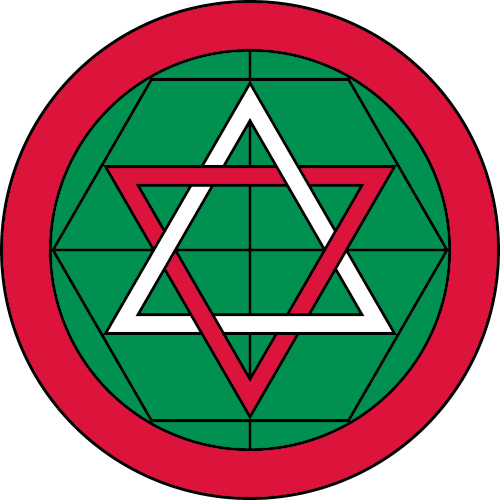
\includegraphics{pantacle.png}};
	\node (One) at (-5,0) {};
	\node (Two) at (5,0) {};
	\def\myshift#1{\raisebox{-2.5ex}}
	\draw [-,thick,black!0,postaction={decorate,decoration={text along path,text align=center,text={|\myshift|B O T T O M T E X T}}}] (One) to [bend right=45]  (Two);
	\def\myshift#1{\raisebox{1ex}}
	\draw [-,thick,black!0,postaction={decorate,decoration={text along path,text align=center,text={|\myshift|T O P \jeheshua{} T E X T}}}] (One) to [bend left=45] (Two);
	\end{tikzpicture}
	
	
\end{document}